\documentclass[aspectratio=169]{beamer}
%[handout]

\usetheme[progressbar=frametitle]{metropolis}
\usepackage{appendixnumberbeamer}

\usepackage[utf8]{inputenc}
\usepackage[T1]{fontenc}

\usepackage[brazil]{babel}
\usepackage[outputdir=..]{minted}
\usepackage{xcolor}
\usepackage{soul} % strikethrough
\usepackage{advdate}
\usepackage{graphicx}
\graphicspath{{figs/}}
\usepackage{graphbox}

\usepackage[ampersand]{easylist}

\usepackage{multirow}
\usepackage{multicol}
\usepackage{subcaption}

\usepackage{pgf,tikz}
\usetikzlibrary{shapes,arrows,positioning}
\usetikzlibrary{circuits.logic.US}
\usetikzlibrary{matrix,calc}

\usepackage{karnaugh-map}

\usepackage{pgfpages}
\setbeameroption{hide notes} % Only slides
% \setbeameroption{show only notes} % Only notes
% \setbeameroption{show notes on second screen=right} % Both

% \graphicspath{{../figs/}}

\definecolor{bgc}{rgb}{0.95,0.9,0.95}
\definecolor{links}{HTML}{2A7F7F}
\hypersetup{colorlinks,linkcolor=,urlcolor=links}

\newminted{verilog}{fontsize=\scriptsize, 
    linenos,
    numbersep=8pt,
    bgcolor=bgc,
    tabsize=4,
    framesep=3mm} 
    %frame=lines,

\newcommand{\verilog}[1]{\verilogf{#1}{\footnotesize}}

\newcommand{\verilogf}[2]{\inputminted[fontsize=#2, 
    linenos,
    tabsize=2,
    numbersep=4pt,
    bgcolor=bgc,
    framesep=3mm]{verilog}{../codes/#1.v}
}

\newminted{nasm}{fontsize=\scriptsize, 
		   linenos,
		   numbersep=8pt,
           bgcolor=bgc,
		   framesep=3mm} 

\usepackage{booktabs}
\usepackage[scale=2]{ccicons}

\usepackage{pgfplots}
\usepgfplotslibrary{dateplot}

\usepackage{hyperref}


\usepackage{xspace}
\newcommand{\themename}{\textbf{\textsc{metropolis}}\xspace}



\usepackage{pifont}% http://ctan.org/pkg/pifont
\newcommand{\cmark}{\ding{51}}%
\newcommand{\xmark}{\ding{55}}%

% \tiny	
% \scriptsize
% \footnotesize
% \small	
% \normalsize	
% \large	
% \Large	
% \LARGE	
% \huge	
% \Huge	



\newminted{python}{fontsize=\scriptsize, 
		   linenos,
		   breaklines,
		   numbersep=8pt,
           tabsize=2,
		   framesep=3mm} 
		   
\newminted{verilog}{fontsize=\scriptsize, 
		   linenos,
		   breaklines,
		   numbersep=8pt,
           tabsize=2,
		   framesep=3mm} 
		   




\definecolor{bgc}{rgb}{0.95,0.9,0.95}
\definecolor{links}{HTML}{2A7F7F}
\hypersetup{colorlinks,linkcolor=,urlcolor=links}


% \usepackage[style=apa]{biblatex}
% \addbibresource{mm.bib}


% \author{\large Prof. Ricardo Menotti (\href{mailto:menotti@ufscar.br}{menotti@ufscar.br})}

\newcommand{\newauthor}[2]{
  \parbox{0.50\textwidth}{
    \texorpdfstring
      {
        \centering
        \small #1 \newline
        {\scriptsize{\urlstyle{same}\href{mailto:#2}{#2}\urlstyle{tt}}}
      }
      {#1} \newline
  }
}

\author{
  \newauthor{Prof. Ricardo Menotti}{menotti@ufscar.br}
\and \newauthor{Prof. Luciano de Oliveira Neris}{lneris@ufscar.br}  
%\and \newauthor{Prof. Artino Quintino da Silva Filho}{artino@ufscar.br}
% \and \newauthor{Prof. Maurício Figueiredo}{mauricio@ufscar.br}
% \and \newauthor{Prof. Edilson Kato}{kato@ufscar.br}
% \and \newauthor{Prof. Roberto Inoue}{rsinoue@ufscar.br}
}

\date{Atualizado em: \today}

\institute{\large \textbf{Departamento de Computação} \\
Centro de Ciências Exatas e de Tecnologia \\
Universidade Federal de São Carlos}

\title{Lógica Digital (1001351)}

\titlegraphic{\hfill
\includegraphics[height=1.5cm]{LogoUfscar}}



\setbeameroption{hide notes} % Only slides
%\setbeameroption{show only notes} % Only notes
% \setbeameroption{show notes on second screen=right} % Both
% See: https://gist.github.com/andrejbauer/ac361549ac2186be0cdb

\subtitle{Algebra Booleana} % 

\begin{document}

\begin{frame}
	\titlepage
\end{frame} 

% Uncomment if you want a summary slide
% \begin{frame}{Conteúdo}
% 	\tableofcontents
% \end{frame}

\section{Algebra Booleana}

\frame{
	\frametitle{\insertsection}
	\begin{itemize}
		\item Publicada em 1849 por George Boole;
		\item Claude Shannon demonstrou sua utilidade para a descrição de circuitos no final da década de 1930;
		\item Deste então, constitui a base para a tecnologia digital moderna. 
	\end{itemize}
}


\section{Axiomas}

\frame{
\frametitle{Axiomas}
\begin{columns}
\begin{column}[c]{5cm}
	\begin{itemize}
		\item<1->  1a \hspace{0.2cm} $0 . 0 = 0$
		\item<2->  2a \hspace{0.2cm} $1 . 1 = 1$
		\item<3->  3a \hspace{0.2cm} $0 . 1 =  1 . 0 = 0$
		\item<4->  4a \hspace{0.2cm} Se $x = 0$, então $\overline{x} = 1$  
	\end{itemize}
\end{column}
\begin{column}[c]{5cm}
	\begin{itemize}
		\item<1->  1b \hspace{0.2cm} $1 + 1 = 1$ 
		\item<2->  2b \hspace{0.2cm} $0 + 0 = 0$
		\item<3->  3b \hspace{0.2cm} $1 + 0 =  0 + 1 = 1$
		\item<4->  4b \hspace{0.2cm} Se $x = 1$, então $\overline{x} = 0$  
	\end{itemize}
\end{column}
\end{columns}

}

\section{Teoremas}

\frame{
\frametitle{Teoremas com uma variável}
\begin{columns}
\begin{column}[c]{5cm}
	\begin{itemize}
		\item<1-> 5a \hspace{0.2cm} $x . 0 = 0$
		\item<2-> 6a \hspace{0.2cm} $x . 1 = x$ 
		\item<3-> 7a \hspace{0.2cm} $x . x = x$
		\item<4-> 8a \hspace{0.2cm} $x . \overline{x} = 0$
	\end{itemize}
\end{column}
\begin{column}[c]{5cm}
	\begin{itemize}
		\item<1-> 5b \hspace{0.2cm} $x + 1 = 1$
		\item<2-> 6b \hspace{0.2cm} $x + 0 = x$ 
		\item<3-> 7b \hspace{0.2cm} $x + x = x$
		\item<4-> 8b \hspace{0.2cm} $x + \overline{x} = 1$
	\end{itemize}
\end{column}
\end{columns}
\begin{columns}
\begin{column}[c]{5cm}
	\begin{itemize}
		\item<5-> 9~~\,\hspace{0.2cm} $\overline{\overline{x}}$ = $x$
	\end{itemize}
\end{column}
\begin{column}[c]{5cm}
\end{column}
\end{columns}
}

\frame{
\frametitle{Princípio da dualidade}
    Dada uma expressão lógica, sua \em{dual} pode ser obtida trocando-se todos os operadores + por ., e vice versa, e trocando todos os 0s por 1s, e vice versa. 
}

\frame{
\frametitle{Propriedades}

\textbf{Comutativas}
\begin{columns}
\begin{column}[c]{5cm}
	\begin{itemize}
		\item<1-> 10a \hspace{0.2cm} $x . y = y . x$
	\end{itemize}
\end{column}
\begin{column}[c]{5cm}
	\begin{itemize}
		\item<1-> 10b \hspace{0.2cm} $x + y = y + x$
	\end{itemize}
\end{column}
\end{columns}

\vspace{5mm}

\pause \textbf{Associativas}
\begin{columns}
\begin{column}[c]{5cm}
	\begin{itemize}
		\item<1-> 11a \hspace{0.2cm} $x . (y . z) = (x . y) . z$
	\end{itemize}
\end{column}
\begin{column}[c]{5cm}
	\begin{itemize}
		\item<1-> 11b \hspace{0.2cm} $x + (y + z) = (x + y) + z$
	\end{itemize}
\end{column}
\end{columns}


\vspace{5mm}

\pause \textbf{Distributivas}
\begin{columns}
\begin{column}[c]{5cm}
	\begin{itemize}
		\item<1-> 12a \hspace{0.2cm} $x . ( y + z ) = x . y + x . z$
	\end{itemize}
\end{column}
\begin{column}[c]{5cm}
	\begin{itemize}
		\item<1-> 12b \hspace{0.2cm} $x + y . z = (x + y) . (x + z)$
	\end{itemize}
\end{column}
\end{columns}

}


\frame{
\frametitle{Propriedades}

\textbf{Absorção}
\begin{columns}
\begin{column}[c]{5cm}
	\begin{itemize}
		\item<1-> 13a \hspace{0.2cm} $x + x . y = x$
	\end{itemize}
\end{column}
\begin{column}[c]{5cm}
	\begin{itemize}
		\item<1-> 13b \hspace{0.2cm} $x . (x + y) = x$
	\end{itemize}
\end{column}
\end{columns}

\vspace{5mm}

\pause \textbf{Combinação}
\begin{columns}
\begin{column}[c]{5cm}
	\begin{itemize}
		\item<1-> 14a \hspace{0.2cm} $x . y + x . \overline{y} = x$
	\end{itemize}
\end{column}
\begin{column}[c]{5cm}
	\begin{itemize}
		\item<1-> 14b \hspace{0.2cm} $(x + y) . (x + \overline{y}) = x$
	\end{itemize}
\end{column}
\end{columns}


\vspace{5mm}

\pause \textbf{DeMorgan}
\begin{columns}
\begin{column}[c]{5cm}
	\begin{itemize}
		\item<1-> 15a \hspace{0.2cm} $\overline{x . y} = \overline{x} + \overline{y}$
		\item<1-> 16a \hspace{0.2cm} $x + \overline{x} . y = x + y$
	\end{itemize}
\end{column}
\begin{column}[c]{5cm}
	\begin{itemize}
		\item<1-> 15b \hspace{0.2cm} $\overline{x + y} = \overline{x} . \overline{y}$
		\item<1-> 16b \hspace{0.2cm} $x . (\overline{x} + y) = x . y$
	\end{itemize}
\end{column}
\end{columns}

}

\frame{     \centering
    \frametitle{Prova por tabela verdade}
    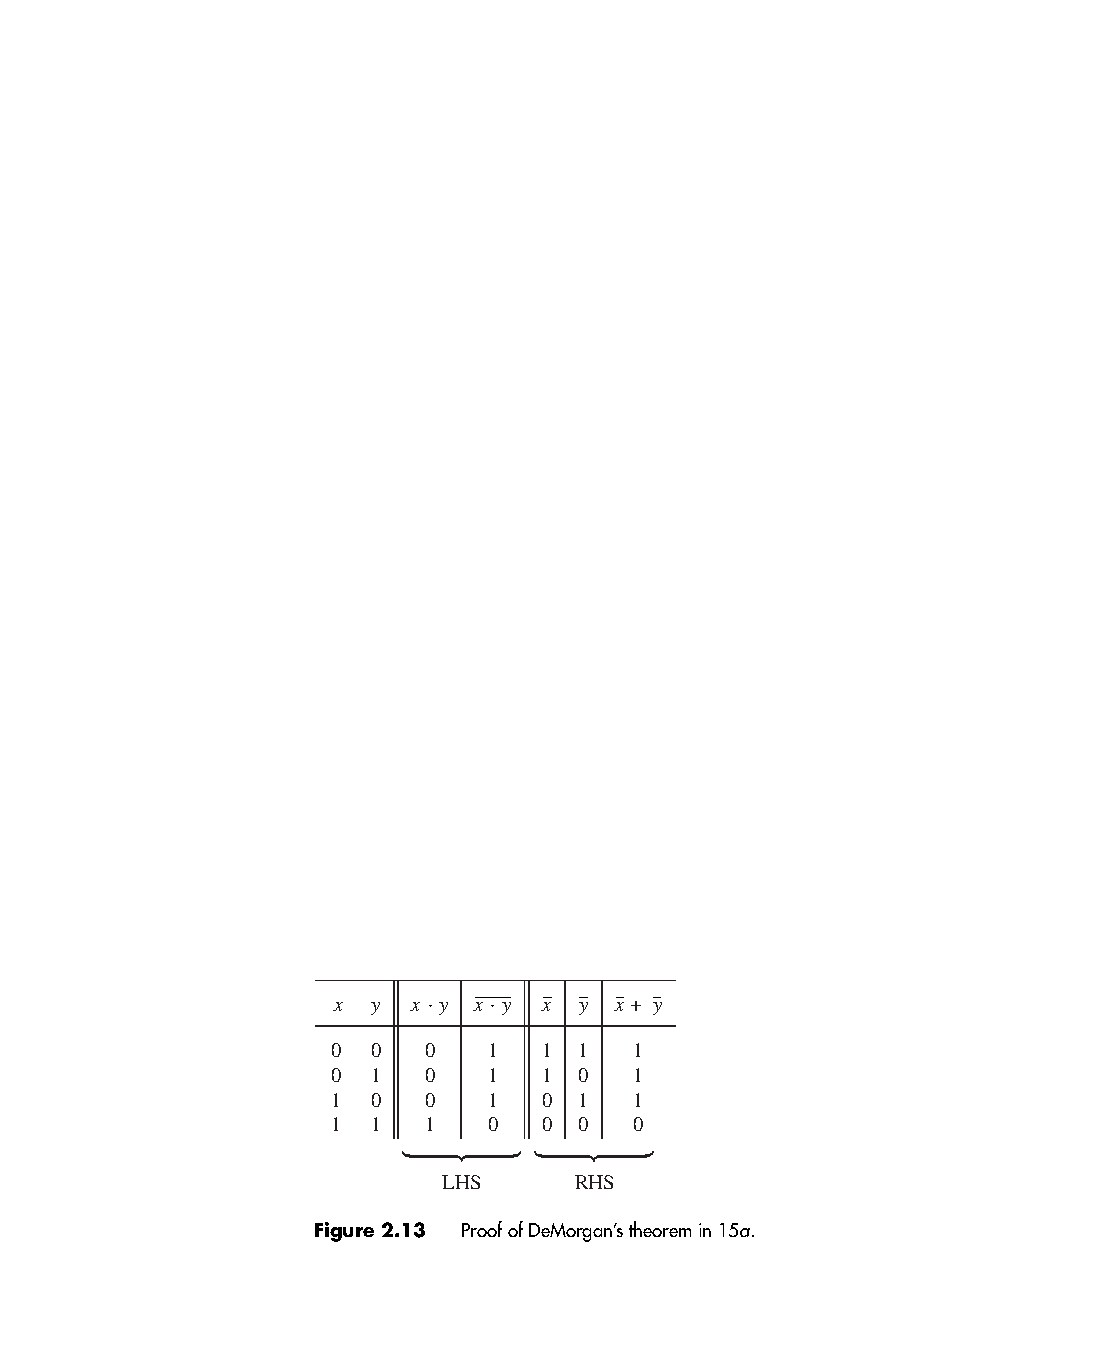
\includegraphics[width=.7\textwidth]{VerilogFig2_13}
}

\frame{    
    \frametitle{Prova por manipulação algébrica}
	Vamos provar a validade da expressão: \hfill \\
	\vspace{0.1cm}
	\hfill $(x_1+x_3).(\overline{x}_1+\overline{x}_3)=x_1.\overline{x}_3+\overline{x}_1.x_3$ \\
	\vspace{0.1cm}
	\pause
	O lado esquerdo pode ser manipulado usando a propriedade distributiva (12a):\hfill \\
	\vspace{0.1cm}
	\pause
	\hfill $LHS=(x_1+x_3).\overline{x}_1+(x_1+x_3).\overline{x}_3$\\
	\vspace{0.1cm}
	\pause
	Aplicando novamente a mesma propriedade:\hfill \\
	\vspace{0.1cm}
	\pause
	\hfill $LHS=x_1.\overline{x}_1+x_3.\overline{x}_1+x_1.\overline{x}_3+x_3.\overline{x}_3$\\
	\vspace{0.1cm}
	\pause
	De acordo com o teorema 8a, os termos $x_1.\overline{x}_1$ e $x_3.\overline{x}_3$ são ambos iguais a $0$, portanto:\hfill \\
	\vspace{0.1cm}
	\pause
	\hfill $LHS=0+x_3.\overline{x}_1+x_1.\overline{x}_3+0$\\
	\vspace{0.1cm}
	\pause
	A partir do teorema 6b temos:\hfill \\
	\pause
	\vspace{0.1cm}
	\hfill $LHS=x_3.\overline{x}_1+x_1.\overline{x}_3$\\
	\vspace{0.1cm}
	\pause
	Usando as propriedades comutativas 10a e 10b, temos:\hfill \\
	\vspace{0.1cm}
	\pause
	\hfill $LHS=x_1.\overline{x}_3+\overline{x}_1.x_3$ \\ 
}


\frame{    
    \frametitle{Prova por manipulação algébrica}
    \begin{tabular}{rcl}
	$(x_1+x_3).(\overline{x}_1+\overline{x}_3)$ & $=$ & $x_1.\overline{x}_3+\overline{x}_1.x_3$ \\
	$LHS$ & $=$ & $(x_1+x_3).\overline{x}_1+(x_1+x_3).\overline{x}_3$\\
	$LHS$ & $=$ & $x_1.\overline{x}_1+x_3.\overline{x}_1+x_1.\overline{x}_3+x_3.\overline{x}_3$\\
	$LHS$ & $=$ & $0+x_3.\overline{x}_1+x_1.\overline{x}_3+0$\\
	$LHS$ & $=$ & $x_3.\overline{x}_1+x_1.\overline{x}_3$\\
	$LHS$ & $=$ & $x_1.\overline{x}_3+\overline{x}_1.x_3$ \\ 
	\end{tabular}
}

\frame{    
    \frametitle{Prova por manipulação algébrica}
    Considerando a equação:\\
	\vspace{0.1cm}
    \hspace*{0pt}\hfill $x_1.\overline{x}_3+\overline{x}_2.\overline{x}_3+x_1.x_3+\overline{x}_2.x_3=\overline{x}_1.\overline{x}_2+x_1.x_2+x_1.\overline{x_2}$ \\
	\vspace{0.1cm}
	\only<2->{O lado esquerdo pode ser manipulado assim:}
	\vspace{0.1cm}
	\begin{tabular}{rll}
	\only<3->{	$LHS =$ & $x_1.\overline{x}_3+x_1.x_3+\overline{x}_2.\overline{x}_3+\overline{x}_2.x_3$ & usando 10b \\}
	\only<4->{	$    =$ & $x_1.(\overline{x}_3+x_3)+\overline{x}_2.(\overline{x}_3+x_3)$ & usando 12a \\}
	\only<5->{	$    =$ & $x_1.1+\overline{x}_2.1$ & usando 8b \\}
	\only<6->{	$    =$ & $x_1+\overline{x}_2$ & usando 6a \\}
	\end{tabular} \\
	\vspace{0.1cm}
	\only<7->{O lado direito pode ser manipulado assim:}
	\vspace{0.1cm}
	\begin{tabular}{rll}
	\only<8->{   $RHS =$ & $\overline{x}_1.\overline{x}_2+x_1.(x_2+\overline{x_2})$ & usando 12a\\}
	\only<9->{   $    =$ & $\overline{x}_1.\overline{x}_2+x_1.1$ & usando 8b\\}
	\only<10->{   $    =$ & $\overline{x}_1.\overline{x}_2+x_1$ & usando 6a\\}
	\only<11->{   $    =$ & $x_1+\overline{x}_1.\overline{x}_2$ & usando 10b\\}
	\only<12->{   $    =$ & $x_1+\overline{x}_2$ & usando 16a\\}
	\end{tabular}
}

\frame{
\frametitle{Precedência das operações}
    Parênteses podem ser usados para indicar a ordem das operações. Na ausência deles, as operações devem ser resolvidas na ordem: NÃO, E e OU. \\
    Portanto, \\
     \hspace*{0pt}\hfill $(x_1 . x_2) + ((\overline{x}_1) . (\overline{x}_2))$ \\
    pode ser escrita na forma \\
     \hspace*{0pt}\hfill $x_1 . x_2 + \overline{x}_1 . \overline{x}_2$ \\
    ou ainda \\
     \hspace*{0pt}\hfill $x_1 x_2 + \overline{x}_1 \overline{x}_2$ \\
    omitindo-se o operador . 
}

\section{Exemplos}

\frame{
\frametitle{Provar que:}
\begin{scriptsize}

$(x_{1}+x_{2}).(x_{2}+x_{3}).(\overline{x}_{1}+\overline{x}_{3})=
x_{1}.x_{2}.\overline{x}_{3}+\overline{x}_{1}.x_{2}+\overline{x}_{1}.x_{2}.x_{3}+x_{2}.\overline{x}_{3}$

\vspace{20pt}
\pause
$LHS=(x_{1}+x_{2}).(x_{2}+x_{3}).(\overline{x}_{1}+\overline{x}_{3})$
\pause
$LHS=x_{1}.(x_{2}+x_{3}).(\overline{x}_{1}+\overline{x}_{3})+
x_{2}.(x_{2}+x_{3}).(\overline{x}_{1}+\overline{x}_{3})$
\pause
$LHS=x_{1}.(x_{2}+x_{3}).\overline{x}_{1}+
x_{1}.(x_{2}+x_{3}).\overline{x}_{3}+
x_{2}.(x_{2}+x_{3}).\overline{x}_{1}+
x_{2}.(x_{2}+x_{3}).\overline{x}_{3}$
\pause
$LHS=x_{1}.\overline{x}_{1}.(x_{2}+x_{3})+
x_{1}.\overline{x}_{3}.(x_{2}+x_{3})+
x_{2}.\overline{x}_{1}.(x_{2}+x_{3})+
x_{2}.\overline{x}_{3}.(x_{2}+x_{3})$
\pause
$LHS=x_{1}.\overline{x}_{1}.x_{2}+
x_{1}.\overline{x}_{1}.x_{3}+
x_{1}.\overline{x}_{3}.x_{2}+
x_{1}.\overline{x}_{3}.x_{3}+
x_{2}.\overline{x}_{1}.x_{2}+
x_{2}.\overline{x}_{1}.x_{3}+
x_{2}.\overline{x}_{3}.x_{2}+
x_{2}.\overline{x}_{3}.x_{3}$
\pause
$LHS=x_{1}.\overline{x}_{1}.x_{2}+
x_{1}.\overline{x}_{1}.x_{3}+
x_{1}.x_{2}.\overline{x}_{3}+
x_{1}.x_{3}.\overline{x}_{3}+
\overline{x}_{1}.x_{2}.x_{2}+
\overline{x}_{1}.x_{2}.x_{3}+
x_{2}.x_{2}.\overline{x}_{3}+
x_{2}.x_{3}.\overline{x}_{3}$
\pause
$LHS=0.x_{2}+0.x_{3}+
x_{1}.x_{2}.\overline{x}_{3}+
x_{1}.0+
\overline{x}_{1}.x_{2}.x_{2}+
\overline{x}_{1}.x_{2}.x_{3}+
x_{2}.x_{2}.\overline{x}_{3}+
x_{2}.0$
\pause
$LHS=0+0+
x_{1}.x_{2}.\overline{x}_{3}+0+
\overline{x}_{1}.x_{2}.x_{2}+
\overline{x}_{1}.x_{2}.x_{3}+
x_{2}.x_{2}.\overline{x}_{3}+0$
\pause
$LHS=x_{1}.x_{2}.\overline{x}_{3}+
\overline{x}_{1}.x_{2}.x_{2}+
\overline{x}_{1}.x_{2}.x_{3}+
x_{2}.x_{2}.\overline{x}_{3}$
\pause
$LHS=x_{1}.x_{2}.\overline{x}_{3}+
\overline{x}_{1}.x_{2}+
\overline{x}_{1}.x_{2}.x_{3}+
x_{2}.\overline{x}_{3}$

\end{scriptsize}
}

\frame{
\frametitle{Provar que:}
\begin{tiny}
$x.\overline{z} + \overline{x}.z + y.\overline{z}.w = x.\overline{z} + \overline{x}.z + \overline{x}.y.w$

\vspace{20pt}

\pause

$LHS = x.\overline{z} + \overline{x}.z + y.\overline{z}.w$

\pause

$LHS = x.\overline{z}.y+x.\overline{z}.\overline{y}+\overline{x}.z.y+\overline{x}.z.\overline{y}+y.\overline{z}.w$

\pause

$LHS = x.\overline{z}.y.w+
x.\overline{z}.y.\overline{w}+
x.\overline{z}.\overline{y}.w+
x.\overline{z}.\overline{y}.\overline{w}+
\overline{x}.z.y.w+
\overline{x}.z.y.\overline{w}+
\overline{x}.z.\overline{y}.w+
\overline{x}.z.\overline{y}.\overline{w}+
y.\overline{z}.w.x+
y.\overline{z}.w.\overline{x}$

\pause

$LHS = x.y.\overline{z}.w+
x.y.\overline{z}.\overline{w}+
x.\overline{y}.\overline{z}.w+
x.\overline{y}.\overline{z}.\overline{w}+
\overline{x}.y.z.w+
\overline{x}.y.z.\overline{w}+
\overline{x}.\overline{y}.z.w+
\overline{x}.\overline{y}.z.\overline{w}+
x.y.\overline{z}.w+
\overline{x}.y.\overline{z}.w$

\pause

$LHS = $
$x.y.\overline{z}.w+$
$x.y.\overline{z}.\overline{w}+$
$x.\overline{y}.\overline{z}.w+$
$x.\overline{y}.\overline{z}.\overline{w}+$
$\overline{x}.y.z.w+$
$\overline{x}.y.z.\overline{w}+$
$\overline{x}.\overline{y}.z.w+$
$\overline{x}.\overline{y}.z.\overline{w}+$
$\overline{x}.y.\overline{z}.w$

\vspace{20pt}

\pause

$RHS = x.\overline{z} + \overline{x}.z + \overline{x}.y.w$

\pause

$RHS = $
$x.\overline{z}.y + x.\overline{z}.\overline{y} + \overline{x}.z.y+$ $\overline{x}.z.\overline{y} + \overline{x}.y.w$

\pause

$RHS = $
$x.\overline{z}.y.w+$
$x.\overline{z}.y.\overline{w}+$
$x.\overline{z}.\overline{y}.w+$
$x.\overline{z}.\overline{y}.\overline{w}+$
$\overline{x}.z.y.w+$
$\overline{x}.z.y.\overline{w}+$
$\overline{x}.z.\overline{y}.w+$
$\overline{x}.z.\overline{y}.\overline{w}+$
$\overline{x}.y.w.z+$
$\overline{x}.y.w.\overline{z}$

\pause

$RHS = $
$x.y.\overline{z}.w+$
$x.y.\overline{z}.\overline{w}+$
$x.\overline{y}.\overline{z}.w+$
$x.\overline{y}.\overline{z}.\overline{w}+$
$\overline{x}.y.z.w+$   
$\overline{x}.y.z.\overline{w}+$
$\overline{x}.\overline{y}.z.w+$
$\overline{x}.\overline{y}.z.\overline{w}+$
$\overline{x}.y.z.w+$
$\overline{x}.y.\overline{z}.w$

\pause

$RHS = $
$x.y.\overline{z}.w+$
$x.y.\overline{z}.\overline{w}+$
$x.\overline{y}.\overline{z}.w+$
$x.\overline{y}.\overline{z}.\overline{w}+$
$\overline{x}.y.z.w+$
$\overline{x}.y.z.\overline{w}+$
$\overline{x}.\overline{y}.z.w+$
$\overline{x}.\overline{y}.z.\overline{w}+$
$\overline{x}.y.\overline{z}.w$

\end{tiny}
}

\section{Bibliografia} %%%%%%%

\begin{frame}{\insertsection} 
	\begin{itemize}
		\item \href{https://www.google.com.br/search?q=filetype\%3Apdf+Fundamentals+of+Digital+Logic+with+Verilog+Design+&oq=filetype\%3Apdf}{Brown, S. \& Vranesic, Z. - Fundamentals of Digital Logic with Verilog Design, 3rd Ed., Mc Graw Hill, 2009}
		\item \href{https://archive.org/details/investigationofl00boolrich/page/n4}{https://archive.org/details/investigationofl00boolrich/page/n4}
	\end{itemize}
\end{frame}

\begin{frame}
	\titlepage
\end{frame} 

\end{document}